\section{Background \& Motivation}

Greenhouse gas emission from human activities is the main cause of climate
change, which has dire consequences on human health and safety due to extreme
weather events and the overall impact on food production
\cite{mcmichael_global_2004}. Poor people are especially vulnerable because
they do not have the resources to manage or mitigate the impacts of climate
change. For instance, they are more affected by local disruptions in food
supply and natural disasters, have poorer access to healthcare and financial
resources to recover from setbacks \cite{hallegatte_shock_2016}. Many countries
have since pledged to meet the net-zero carbon emissions goal by 2050 and limit
the rise in global temperatures to 1.5$^{\circ}$C \cite{iea_net_2021}.

The transition to a carbon-free economy requires drastic changes in the way
every sector produces or consumes energy in the form of electricity or heat.
The \gls{IEA} published a report, titled ``Net Zero by 2050 - A Roadmap for the
Global Energy Sector'', to set out guidelines to inform policy makers how the
\gls{NZE} could be reached in a way that ``maximizes technical feasibility,
cost-effectiveness and social acceptance, while ensuring continued economic
growth and secure energy supplies''. The \gls{NZE} roadmap projects that
solar \gls{PV} and wind has to make up just under 70\% of
electricity generated globally in 2050 (Figure \ref{fig:2050-elec-source}).
The remaining share largely consists of dispatchable sources, such as
hydropower, carbon-neutral biofuel, and nuclear, since solar \gls{PV} and wind
are non-dispatchable sources which experience daily and seasonal variations in
electricity production. These variations are already causing major shifts in
the electricity markets today. California, a region with high renewable energy
penetration, experienced negative electricity prices during the midday (Figure
\ref{fig:cali-prices}) due to the excess electricity generation from solar
\glspl{PV} and base-load suppliers paying to keep their power plants online to
ramp up for the evening demand spike \cite{forsberg_market_2020}.

\begin{figure}[htb!]
	\centering
	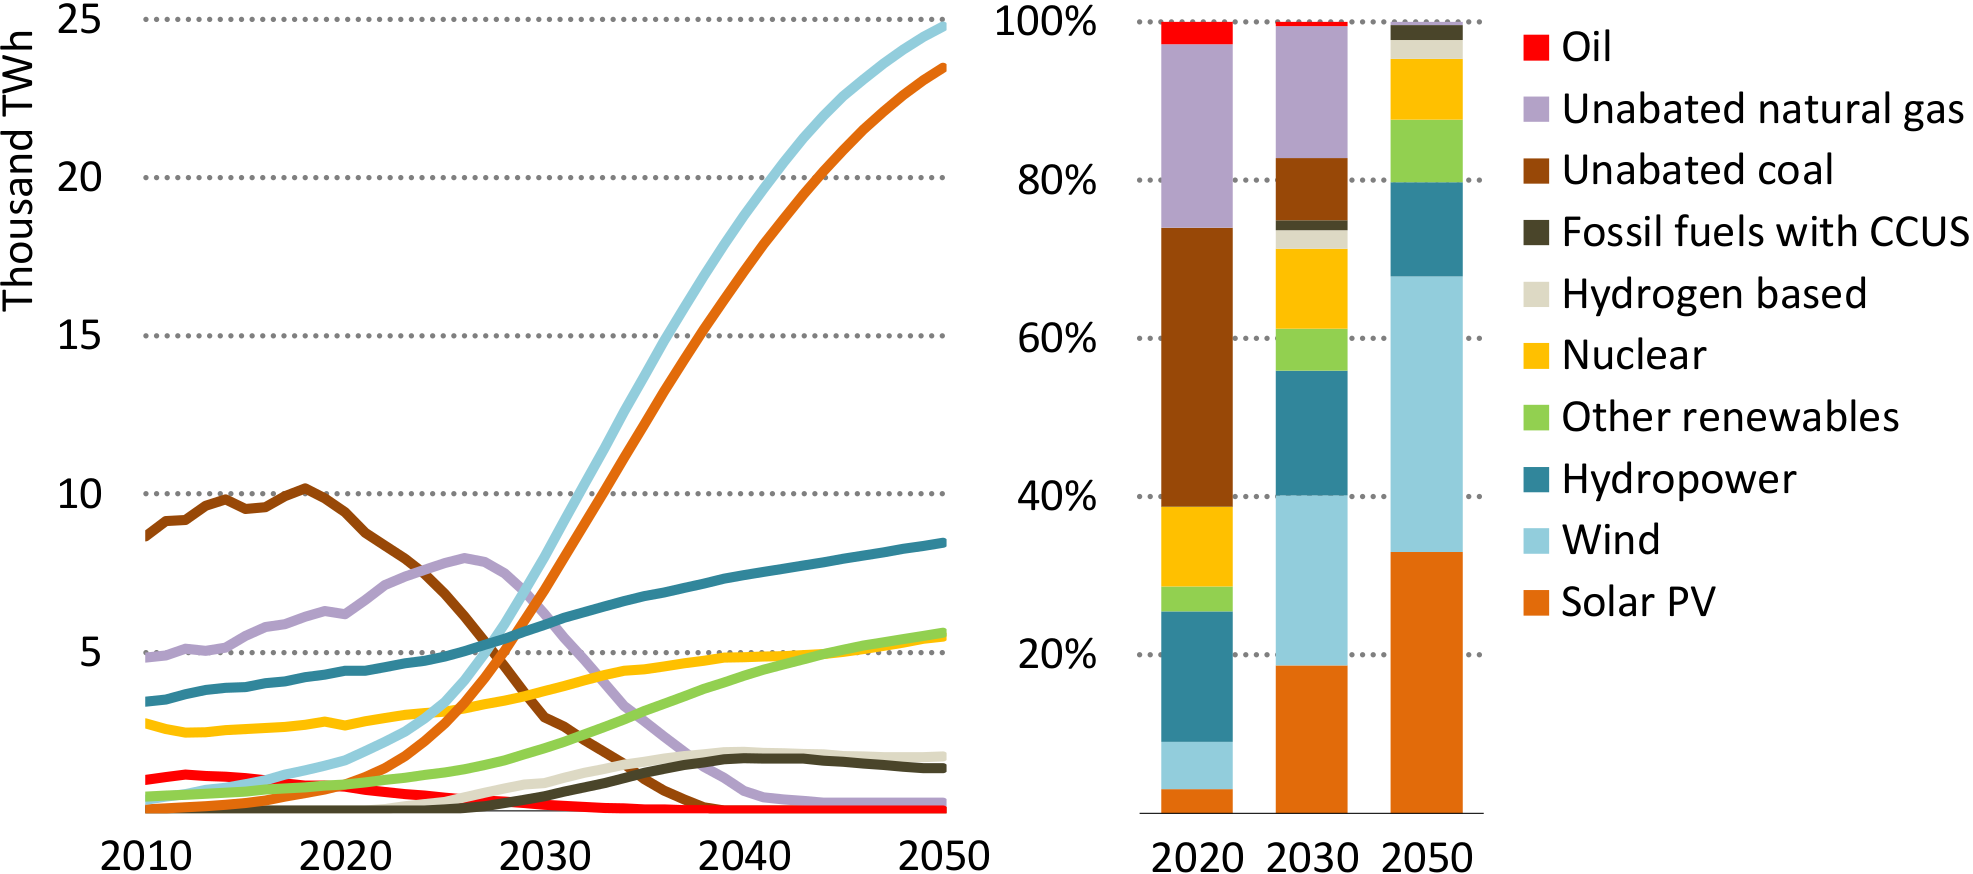
\includegraphics[width=.8\columnwidth]{2050-elec-source}
	\caption{Projected global electricity generation by source in the
	\gls{NZE}. Retrieved from \cite{iea_net_2021}.}
	\label{fig:2050-elec-source}
\end{figure}

\begin{figure}[htb!]
	\centering
	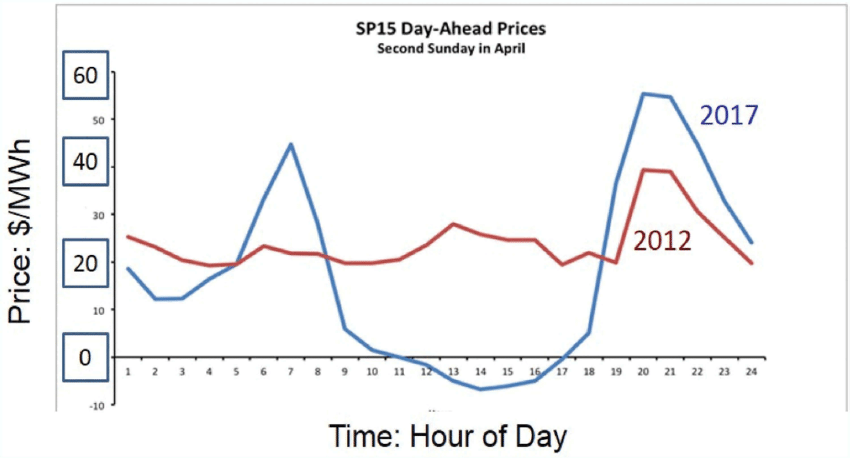
\includegraphics[width=.7\columnwidth]{california-prices}
	\caption{Wholesale electricity prices over 24 hours from the second Sundays
	in April in 2012 and 2017. Retrieved from \cite{forsberg_market_2020}.}
	\label{fig:cali-prices}
\end{figure}

Unlike solar or wind power, nuclear power provides consistent and reliable
power independent of weather conditions. The \gls{NZE} roadmap acknowledges the
need for nuclear power as one of the various dispatchable energy sources;
Figure \ref{fig:2050-elec-source}, taken from the \gls{IEA} \gls{NZE} report,
shows that nuclear power will continue to play an important role in reducing
carbon emissions with electricity generation in 2050 from nuclear projected to
be double the output in 2020 while maintaining an approximate 10\% share in
electricity generation as global energy demand rises. A separate study from
\gls{MIT} \cite{petti_future_2018} reports that attempting to limit carbon
emissions without nuclear power would cause electricity generation costs to
increase significantly due to the disproportionately large excess capacity in
solar \gls{PV}, wind, and battery storage required to maintain electricity
security during periods of adverse weather conditions.
Beyond the electricity sector, nuclear power also has the potential to replace
fossil fuels to meet energy demands from industrial process heat applications
and transportation \cite{forsberg_market_2020}. Solar \gls{PV} and
wind are ill-suited for meeting heat demand such as district heating and
industrial heat applications at economically competitive rates. Some advanced
reactors such as \glspl{MSR} and \glspl{HTGR} operate at sufficiently
high temperatures for chemical, petrochemical, steel, and other industries.
These industries include hydrogen and ammonia production, two hydrogen-based
fuel candidates for replacing fossil fuel consumption in the aviation and
marine sectors to reduce carbon emissions.

The world would have to ramp up the current rate of reactor deployments to
replace aging reactors and displace a portion of the presently large share of
energy production from fossil fuels. However, several obstacles stand in the
way of new reactor deployments. These obstacles include perceived
safety risks, sustainability concerns,
and the ability to compete economically with other sources of energy
\cite{massachusetts_institute_of_technology_future_2003}. A potential solution
to the aforementioned issues is the \gls{MSR} concept, one of six advanced
reactor designs selected by the Generation IV International Forum
\cite{gif_technology_2002} for continued research and development.

\begin{figure}[htb!]
	\centering
	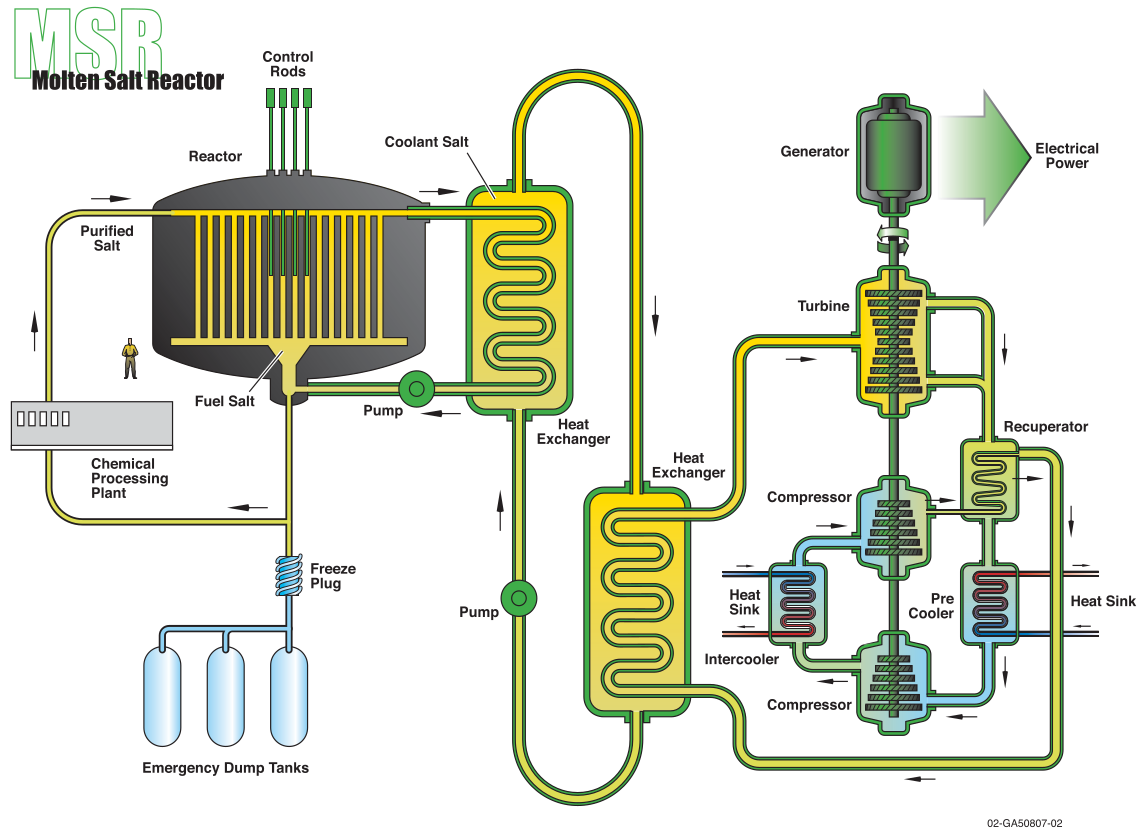
\includegraphics[width=.8\columnwidth]{msr}
	\caption{Schematic diagram of the \gls{MSR} concept. Retrieved from
	\cite{doe_technology_2002}.}
	\label{fig:msr}
\end{figure}

``\glspl{MSR}'' generally refer to all reactor designs that use molten salt as
the primary coolant. In practice, the term usually refers to liquid-fueled
designs which have fissile and/or fertile materials dissolved directly in
molten salt coolants, whereas solid-fueled designs are commonly referred to as
\glspl{FHR}. In this work, I will be following this convention. Figure
\ref{fig:msr} shows a schematic diagram of a typical \gls{MSR}. The fuel salt
refers to the molten salt in the primary coolant loop which carries the fissile
material. Most designs include the intermediate coolant loop illustrated in
Figure \ref{fig:msr} as an additional safety barrier from radioactive release
and to protect the electricity generator section of the plant. \glspl{MSR}
possess an inherently robust
safety feature in the strongly negative fuel temperature coefficient of
reactivity \cite{elsheikh_safety_2013}. This reactivity coefficient limits the
maximum temperature that the reactor core would experience in an accident
scenario such as an unprotected reactivity insertion because the subsequent
rise in core temperatures induces a significant drop in reactivity which
quickly neutralizes the initial reactivity insertion. \glspl{MSR} also
operate at a large thermal margin to boiling and can rely on natural
circulation in the event of a pump failure. As a last resort, some \gls{MSR}
designs incorporate a drain plug consisting of air-cooled frozen salt which
melts when the core temperatures exceed a safety threshold. The hot molten salt
in the core flows down to drain tanks designed to hold the fuel-filled salt in
a subcritical configuration to disrupt any further chain fission reactions.

Some \glspl{MSR} like the \gls{MSBR} or the \gls{MSFR} can
incorporate the thorium fuel cycle for improved sustainability arising from the
use of abundant natural thorium resources and reduced transuranic waste
\cite{heuer_towards_2014}. The latter consequence also reduces economical costs
associated with long-term nuclear waste storage. In addition, the ability to
operate at near atmospheric pressures eliminates the need for a thick pressure
vessel and drives down construction costs, while online fuel reprocessing
reduces reactor downtime during reactor operation \cite{dolan_1_2017}. We can
make further economic arguments supporting \glspl{MSR} in the context of the
carbon-constrained future envisioned in \gls{IEA}'s \gls{NZE} roadmap
\cite{iea_net_2021}. A solar \gls{PV} and wind-dominated energy market produces
variable electricity generation. The resulting volatility in electricity prices
encourages the construction of \textit{heat storage} and \textit{peak power
production} plants. At the same time, demand for carbon-neutral
\textit{hydrogen fuel} will rise as electrification is economically unfeasible
for some industries such as the aviation and marine sectors which depend
energy-dense fuels for transport. As described in
\cite{forsberg_market_2020}, the most cost-efficient options for the
aforementioned resources (\textit{heat storage}, \textit{peak power
production}, and \textit{hydrogen fuel}) all require high-temperature heat.
These factors economically favor salt-cooled reactors over other types of
reactors as they output heat at higher average temperatures.

While \glspl{MSR} have attracted increasing research interest over the past two
decades, they are still very much under research development and no commercial
\gls{MSR} exists yet. Reactor analysis software are essential tools in aiding
reactor development because they help inform design choices and regulations in
line with maximizing safety, reducing proliferation risks, and improving fuel
efficiency. The liquid fuel form in particular introduces new computational
challenges in simulating the transient behavior of \glspl{MSR}. \glspl{MSR}
feature strong negative reactivity feedback in the fuel salt. The feedback
causes strong and near-instantaneous interactions between reactor power and
thermal hydraulic temperature profile. Furthermore, fissile material
and \glspl{DNP} in \glspl{MSR} flow freely within the primary coolant
loop as opposed to being held in place in solid-fuel reactors. The movement of
\glspl{DNP} impacts the effective delayed neutron fraction in the core and
consequently also impacts the transient behavior of the reactor. Therefore,
\gls{MSR} computational models require robust coupling techniques to accurately
capture the strong multiphysics interactions.

Most reactor analysis applications are usually reactor-specific by
design such as TRACE \cite{nrc_trace_2007} for \glspl{LWR}, and
SAS4A/SASSYS-1 \cite{fanning_sas4a/sassys-1_2017} for
liquid metal cooled reactors. Thus, these applications would disregard
\gls{MSR}-specific phenomena and are inappropriate for \gls{MSR}
analysis without modifications to the source code. Some research efforts
do focus on adapting these applications for \gls{MSR} analysis. Examples
include the coupling of modified versions of TRACE and PARCS
\cite{pettersen_coupled_2016}, and the development of VERA-MSR from the
integrated \gls{LWR} simulation tool VERA \cite{graham_development_2019}.
Others developed their \gls{MSR} simulation tools from general
multiphysics or \gls{CFD} applications such as COMSOL
\cite{fiorina_modelling_2014} and OpenFOAM \cite{aufiero_development_2014}.

Similarly, Moltres \cite{lindsay_introduction_2018} is an open-source MSR
simulation tool built in the \gls{MOOSE} \cite{gaston_physics-based_2015}
parallel finite element framework. Lindsay et al.
\cite{lindsay_introduction_2018} first presented the tool in 2017 and
demonstrated its capabilities by simulating 2-D and 3-D models of the
\gls{MSRE}. The results showed good qualitative
agreement with the original design calculations by \gls{MSRE} researchers at
\gls{ORNL}. This thesis presents newer developments in Moltres
allowing for more complex and accurate \gls{MSR} simulations.

\section{Objectives}

This thesis demonstrates latest capabilities of Moltres
\cite{lindsay_introduction_2018}.
In particular, this thesis presents two more recent
developments in Moltres, namely fully integrating \gls{MOOSE}'s incompressible
Navier-Stokes module into Moltres, and introducing a
decay heat model.
The main objective of this thesis is to verify Moltres'
latest capabilities in modeling multiphysics, steady-state, and transient
behavior of fast-spectrum \glspl{MSR} through the study of the \gls{MSFR}
concept. Code-to-code verification is an important exercise in software
development for ensuring that the application produces accurate and reliable
results. This thesis covers the \gls{MSFR} concept mainly because it has been
studied extensively with readily available data in the literature to verify
against. The \gls{MSFR} design also features interesting flow
patterns that greatly affect the steady-state and transient behavior. This
present work will first present a verification of Moltres' \gls{MSFR}
diffusion neutronics against the Monte Carlo neutron transport software
Serpent 2, followed by a verification of
the coupled neutronics/thermal-hydraulics steady-state and accident transient
results against two sets of results published by
Fiorina et al. \cite{fiorina_modelling_2014}. The two sets of results arose
from a collaborative benchmarking exercise by researchers at Politecnico di
Milano and Technical University of Delft with two separate \gls{MSR}
simulation tools. Section \ref{sec:litrev} discusses these tools
in greater detail. The
secondary objective is to identify areas of improvement in Moltres for future
development.

\section{Outline}

The outline of this thesis is as follows. Chapter 2 discusses the history and
features of \glspl{MSR}, and a literature review of existing \gls{MSR}
simulation tools. The chapter also covers the \gls{MSFR} concept in greater
detail. Chapter 3 details the software and the general modeling
approach for generating the results in this thesis. Chapter 4 provides a
neutronics assessment by comparing key neutronics parameters from Moltres'
eigenvalue calculations to Serpent's Monte Carlo calculations. Chapter 5
presents steady-state results of coupled neutronics/thermal-hydraulics
\gls{MSFR} simulations in Moltres. Chapter 6 presents accident transient
simulation results for unprotected reactivity insertions, unprotected loss of
heat sink, unprotected loss of flow, and unprotected pump overspeed. Lastly,
Chapter 7 summarizes the key findings in this thesis
and posits some potential avenues for future work.
